\documentclass[11pt,a4paper,]{article}
\usepackage{lmodern}

\usepackage{amssymb,amsmath}
\usepackage{ifxetex,ifluatex}
\usepackage{fixltx2e} % provides \textsubscript
\ifnum 0\ifxetex 1\fi\ifluatex 1\fi=0 % if pdftex
  \usepackage[T1]{fontenc}
  \usepackage[utf8]{inputenc}
\else % if luatex or xelatex
  \usepackage{unicode-math}
  \defaultfontfeatures{Ligatures=TeX,Scale=MatchLowercase}
\fi
% use upquote if available, for straight quotes in verbatim environments
\IfFileExists{upquote.sty}{\usepackage{upquote}}{}
% use microtype if available
\IfFileExists{microtype.sty}{%
\usepackage[]{microtype}
\UseMicrotypeSet[protrusion]{basicmath} % disable protrusion for tt fonts
}{}
\PassOptionsToPackage{hyphens}{url} % url is loaded by hyperref
\usepackage[unicode=true]{hyperref}
\hypersetup{
            pdftitle={Predicting Critical Elements in Coal Mine Waste: A Machine Learning and Spatial Statistics Approach for a Low-Emission Future},
            pdfborder={0 0 0},
            breaklinks=true}
\urlstyle{same}  % don't use monospace font for urls
\usepackage{geometry}
\geometry{a4paper, centering, text={16cm,25cm}}
\usepackage[style=authoryear-comp,]{biblatex}
\addbibresource{references.bib}
\usepackage{longtable,booktabs}
% Fix footnotes in tables (requires footnote package)
\IfFileExists{footnote.sty}{\usepackage{footnote}\makesavenoteenv{long table}}{}
\IfFileExists{parskip.sty}{%
\usepackage{parskip}
}{% else
\setlength{\parindent}{0pt}
\setlength{\parskip}{6pt plus 2pt minus 1pt}
}
\setlength{\emergencystretch}{3em}  % prevent overfull lines
\providecommand{\tightlist}{%
  \setlength{\itemsep}{0pt}\setlength{\parskip}{0pt}}
\setcounter{secnumdepth}{0}

% set default figure placement to htbp
\makeatletter
\def\fps@figure{htbp}
\makeatother


\title{Predicting Critical Elements in Coal Mine Waste: A Machine Learning and Spatial Statistics Approach for a Low-Emission Future}

%% MONASH STUFF

%% CAPTIONS
\RequirePackage{caption}
\DeclareCaptionStyle{italic}[justification=centering]
 {labelfont={bf},textfont={it},labelsep=colon}
\captionsetup[figure]{style=italic,format=hang,singlelinecheck=true}
\captionsetup[table]{style=italic,format=hang,singlelinecheck=true}


%% FONT
\RequirePackage{bera}
\RequirePackage[charter,expert,sfscaled]{mathdesign}
\RequirePackage{fontawesome}

%% HEADERS AND FOOTERS
\RequirePackage{fancyhdr}
\pagestyle{fancy}
\rfoot{\Large\sffamily\raisebox{-0.1cm}{\textbf{\thepage}}}
\makeatletter
\lhead{\textsf{\expandafter{\@title}}}
\makeatother
\rhead{}
\cfoot{}
\setlength{\headheight}{15pt}
\renewcommand{\headrulewidth}{0.4pt}
\renewcommand{\footrulewidth}{0.4pt}
\fancypagestyle{plain}{%
\fancyhf{} % clear all header and footer fields
\fancyfoot[C]{\sffamily\thepage} % except the center
\renewcommand{\headrulewidth}{0pt}
\renewcommand{\footrulewidth}{0pt}}

%% MATHS
\RequirePackage{bm,amsmath}
\allowdisplaybreaks

%% GRAPHICS
\RequirePackage{graphicx}
\setcounter{topnumber}{2}
\setcounter{bottomnumber}{2}
\setcounter{totalnumber}{4}
\renewcommand{\topfraction}{0.85}
\renewcommand{\bottomfraction}{0.85}
\renewcommand{\textfraction}{0.15}
\renewcommand{\floatpagefraction}{0.8}


%\RequirePackage[section]{placeins}

%% SECTION TITLES


%% SECTION TITLES
\RequirePackage[compact,sf,bf]{titlesec}
\titleformat*{\section}{\Large\sf\bfseries\color[rgb]{0.7,0,0}}
\titleformat*{\subsection}{\large\sf\bfseries\color[rgb]{0.7,0,0}}
\titleformat*{\subsubsection}{\sf\bfseries\color[rgb]{0.7,0,0}}
\titlespacing{\section}{0pt}{2ex}{.5ex}
\titlespacing{\subsection}{0pt}{1.5ex}{0ex}
\titlespacing{\subsubsection}{0pt}{.5ex}{0ex}


%% TITLE PAGE
\def\Date{\number\day}
\def\Month{\ifcase\month\or
 January\or February\or March\or April\or May\or June\or
 July\or August\or September\or October\or November\or December\fi}
\def\Year{\number\year}

%% LINE AND PAGE BREAKING
\sloppy
\clubpenalty = 10000
\widowpenalty = 10000
\brokenpenalty = 10000
\RequirePackage{microtype}

%% PARAGRAPH BREAKS
\setlength{\parskip}{1.4ex}
\setlength{\parindent}{0em}

%% HYPERLINKS
\RequirePackage{xcolor} % Needed for links
\definecolor{darkblue}{rgb}{0,0,.6}
\RequirePackage{url}

\makeatletter
\@ifpackageloaded{hyperref}{}{\RequirePackage{hyperref}}
\makeatother
\hypersetup{
     citecolor=0 0 0,
     breaklinks=true,
     bookmarksopen=true,
     bookmarksnumbered=true,
     linkcolor=darkblue,
     urlcolor=blue,
     citecolor=darkblue,
     colorlinks=true}

\usepackage[showonlyrefs]{mathtools}
\usepackage[no-weekday]{eukdate}

%% BIBLIOGRAPHY

\makeatletter
\@ifpackageloaded{biblatex}{}{\usepackage[style=authoryear-comp, backend=biber, natbib=true]{biblatex}}
\makeatother
\ExecuteBibliographyOptions{bibencoding=utf8,minnames=1,maxnames=3, maxbibnames=99,dashed=false,terseinits=true,giveninits=true,uniquename=false,uniquelist=false,doi=false, isbn=false,url=true,sortcites=false}

\DeclareFieldFormat{url}{\texttt{\url{#1}}}
\DeclareFieldFormat[article]{pages}{#1}
\DeclareFieldFormat[inproceedings]{pages}{\lowercase{pp.}#1}
\DeclareFieldFormat[incollection]{pages}{\lowercase{pp.}#1}
\DeclareFieldFormat[article]{volume}{\mkbibbold{#1}}
\DeclareFieldFormat[article]{number}{\mkbibparens{#1}}
\DeclareFieldFormat[article]{title}{\MakeCapital{#1}}
\DeclareFieldFormat[article]{url}{}
%\DeclareFieldFormat[book]{url}{}
%\DeclareFieldFormat[inbook]{url}{}
%\DeclareFieldFormat[incollection]{url}{}
%\DeclareFieldFormat[inproceedings]{url}{}
\DeclareFieldFormat[inproceedings]{title}{#1}
\DeclareFieldFormat{shorthandwidth}{#1}
%\DeclareFieldFormat{extrayear}{}
% No dot before number of articles
\usepackage{xpatch}
\xpatchbibmacro{volume+number+eid}{\setunit*{\adddot}}{}{}{}
% Remove In: for an article.
\renewbibmacro{in:}{%
  \ifentrytype{article}{}{%
  \printtext{\bibstring{in}\intitlepunct}}}

\AtEveryBibitem{\clearfield{month}}
\AtEveryCitekey{\clearfield{month}}

\makeatletter
\DeclareDelimFormat[cbx@textcite]{nameyeardelim}{\addspace}
\makeatother

\author{\sf{\Large\textbf{Yuhao Long}\\\large Master of Business Analytics\newline 33412448 \newline \href{mailto:ylon0012@student.monash.edu}{\nolinkurl{ylon0012@student.monash.edu}}\\[0.5cm]}{\Large\textbf{Evan Ginting}\\\large Master of Business Analytics\newline 33477558 \newline \href{mailto:egin0003@student.monash.edu}{\nolinkurl{egin0003@student.monash.edu}}\\[0.5cm]}}

\date{\sf\Date~\Month~\Year}
\makeatletter
\lfoot{\sf Long, Ginting: \@date}
\makeatother


%%%% PAGE STYLE FOR FRONT PAGE OF REPORTS

\makeatletter
\def\organization#1{\gdef\@organization{#1}}
\def\telephone#1{\gdef\@telephone{#1}}
\def\email#1{\gdef\@email{#1}}
\makeatother
  \organization{ETC5543}

  \def\name{Department of\newline Econometrics \&\newline Business Statistics}

  \telephone{(03) 9905 2478}

  \email{\href{mailto:BusEco-Econometrics@monash.edu}{\nolinkurl{BusEco-Econometrics@monash.edu}}}

\def\webaddress{\url{http://buseco.monash.edu/ebs/consulting/}}
\def\abn{12 377 614 012}
\def\extraspace{\vspace*{1.6cm}}
\makeatletter
\def\contactdetails{\faicon{phone} & \@telephone \\
                    \faicon{envelope} & \@email}
\makeatother

\usepackage[absolute,overlay]{textpos}
\setlength{\TPHorizModule}{1cm}
\setlength{\TPVertModule}{1cm}

%%%% FRONT PAGE OF REPORTS

\def\reporttype{Report for}

\long\def\front#1#2#3{
\newpage
\begin{textblock}{7}(12.7,28.2)\hfill

\includegraphics[height=0.6cm]{AACSB}~~~

\includegraphics[height=0.6cm]{EQUIS}~~~

\includegraphics[height=0.6cm]{AMBA}
\end{textblock}
\begin{singlespacing}
\thispagestyle{empty}
\vspace*{-1.4cm}
\hspace*{-1.4cm}
\hbox to 16cm{
  \hbox to 6.5cm{\vbox to 14cm{\vbox to 25cm{
    
\includegraphics[width=6cm]{monash2}
    \vfill
    
\includegraphics[width=3.5cm]{MBSportrait}
    \vspace{0.4cm}
    \par
    \parbox{6.3cm}{\raggedright
      \sf\color[rgb]{0.00,0.00,0.70}
      {\large\textbf{\name}}\par
      \vspace{.7cm}
      \tabcolsep=0.12cm\sf\small
      \begin{tabular}{@{}ll@{}}\contactdetails
      \end{tabular}
      \vspace*{0.3cm}\par
      ABN: \abn\par
    }
  }\vss}\hss}
  \hspace*{0.2cm}
  \hbox to 1cm{\vbox to 14cm{\rule{1pt}{26.8cm}\vss}\hss\hfill}
  \hbox to 10cm{\vbox to 14cm{\vbox to 25cm{
      \vspace*{3cm}\sf\raggedright
      \parbox{11cm}{\sf\raggedright\baselineskip=1.2cm
         \fontsize{24.88}{30}\color[rgb]{0.70,0.00,0.00}\sf\textbf{#1}}
      \par
      \vfill
      \large
      \vbox{\parskip=0.8cm #2}\par
      \vspace*{2cm}\par
      \reporttype\\[0.3cm]
      \hbox{#3}%\\[2cm]\
      \vspace*{1cm}
      {\large\sf\textbf{\Date~\Month~\Year}}
   }\vss}
  }}
\end{singlespacing}
\newpage
}

\makeatletter
\def\titlepage{\front{\expandafter{\@title}}{\@author}{\@organization}}
\makeatother

\usepackage{setspace}
\setstretch{1.5}

%% Any special functions or other packages can be loaded here.
\usepackage{booktabs}
\usepackage{longtable}
\usepackage{array}
\usepackage{multirow}
\usepackage{wrapfig}
\usepackage{float}
\usepackage{colortbl}
\usepackage{pdflscape}
\usepackage{tabu}
\usepackage{threeparttable}
\usepackage{threeparttablex}
\usepackage[normalem]{ulem}
\usepackage{makecell}
\usepackage{xcolor}


\begin{document}
\titlepage

{
\setcounter{tocdepth}{2}
\tableofcontents
}
\newpage

\hypertarget{abstract}{%
\section{Abstract}\label{abstract}}

\hypertarget{background-and-motivation}{%
\section{Background and Motivation}\label{background-and-motivation}}

\hypertarget{critical-elements-overview}{%
\subsection{Critical Elements Overview}\label{critical-elements-overview}}

In this technology advancement era where mineral-based technologies are relied by many industrial sectors, critical elements become highly-sought elements in the world \autocite{Emsbo2021}. Critical elements can be defined by two main criteria: first, elements that are essential for manufacturing modern technologies, supporting economic frameworks, and ensuring national security; and second, elements with vulnerable supply chains, which can be affected by political issues, geographic concentration of extraction or production, and natural disasters \autocite{Lian2024,Fortier2018,DISR2023}.

According to \href{https://www.industry.gov.au/publications/critical-minerals-strategy-2023-2030}{Critical Minerals Strategy 2023--2030} \autocite{geoscience2023}, Geoscience Australia has identified 15 elements as highly vulnerable to future supply chain disruptions and an additional 15 elements as having moderate risk in Table \ref{tab:celist}(\autocite{Coyne2023}; \autocite{Skirrow2013}; \autocite{IEA2024b}; \autocite{Fortier2018}; \autocite{Austrade2024}). Among these critical elements, Rare-earth elements takes a significant subset in critical element, comprise of 15 element in lanthanoid series and 2 extra elements with similar chemical properties--Scandium(Sc) and Yttrium(Y). Unlike name implication, albeit their overall natural abundance(NA) in earth crust is not extremely rare (average 180-200 ppm) their distribution in earth is quite scattered and strong propensity to coexist in pairs or group within ore deposits in terms of geochemical properties \autocite{Zhou2017}.

Critical elements (including REE) are crucial for many high-tech industries, including electronics, renewable energy, and defense \autocite{Huang2018}. Global initiatives to reduce carbon emissions by transitioning to clean energy have significantly impelled the demand for critical elements, which are essential for achieving this goal \autocite{IEA2021,Wang2022}. According to \textcite{IEA2024} research, demand for these elements is projected to double, triple, or even quadruple, depending on the scenario, relative to current production levels. Among these elements, lithium is experiencing the most rapid growth due to rising demand for electric vehicle (EV) batteries, while copper leads in terms of production volume. Graphite demand is expected to almost quadruple, and the demand for nickel, cobalt, and rare earth elements (REEs) is projected to double. Furthermore, \textcite{Fortier2018} indicates that the growing reliance on critical elements is also driven by their applications across various key sectors, including energy, defense, communications, healthcare, transportation, and agriculture. These dynamics have intensified competition to discover new sources and establish stable, long-term supply chains for these vital resources \autocite{Emsbo2021}. The prominent usage of each element and its projected demand are detailed in Table \ref{tab:celist}.

\begingroup\fontsize{9}{11}\selectfont

\begin{longtabu} to \linewidth {>{\centering}X>{\centering}X>{\centering}X>{\centering}X>{\centering\arraybackslash}p{5cm}>{\centering}X}
\caption{\label{tab:celist}\textbf{Summary of Critical Elements: Production, Global Share, Projected Demand, and Usage}}\\
\toprule
Critical Element & Production (Kilotonnes) \textsuperscript{1} & Global Production (Percentage) & Projected Demand (Kilotonnes) \textsuperscript{2} & Usage \textsuperscript{3} & Level\\
\midrule
\endfirsthead
\caption[]{\label{tab:celist}\textbf{Summary of Critical Elements: Production, Global Share, Projected Demand, and Usage} \textit{(continued)}}\\
\toprule
Critical Element & Production (Kilotonnes) \textsuperscript{1} & Global Production (Percentage) & Projected Demand (Kilotonnes) \textsuperscript{2} & Usage \textsuperscript{3} & Level\\
\midrule
\endhead

\endfoot
\bottomrule
\multicolumn{6}{l}{\rule{0pt}{1em}\textsuperscript{a} Data collected in 2012.}\\
\multicolumn{6}{l}{\rule{0pt}{1em}\textsuperscript{b} 17 elements, including lanthanoid, Scandium (Sc), and Yttrium (Y).}\\
\multicolumn{6}{l}{\rule{0pt}{1em}\textsuperscript{c} 6 elements, including all transition metals in the d-block.}\\
\multicolumn{6}{l}{\rule{0pt}{1em}\textit{Source:} \textsuperscript{1} Skirrow et al., 2013 \& Coyne and Campbell, 2023; \textsuperscript{2} IEA, 2024b; \textsuperscript{3} Fortier et. al., 2018; Austrade, 2024}\\
\endlastfoot
Aluminum and derivative (Al) & 20 & 14 & - & Aerospace alloys, Coating in Li-ion batteries & \cellcolor[HTML]{F7D7DC}{High}\\
Cobalt (Co) & 5.9 & 3 & 243.03 & Li-ion battery cathodes, stainless steels, superalloys & \cellcolor[HTML]{F7D7DC}{High}\\
Gallium (Ga) & - & - & 0.25 & Radar, light-emitting diodes (LEDs), photovoltaics films & \cellcolor[HTML]{F7D7DC}{High}\\
Germanium (Ge) & - & - & 0.03 & Fiber/infrared optics, Polymerization Catalysts, 
          semiconductors & \cellcolor[HTML]{F7D7DC}{High}\\
Lithium(Li) & 61 & 47 & 615.55 & Li-ion batteries, aerospace alloys, ceramics & \cellcolor[HTML]{F7D7DC}{High}\\
\addlinespace
Magnesium(Mg) & 2.6 & 10 & 30.95 & Pyrotechnics, nanocomposites in automotive/aerospace & \cellcolor[HTML]{F7D7DC}{High}\\
Manganese(Mn) & 3.3 & 17 & 855 & Steel, Agricultural fertilizer, lightweight alloys & \cellcolor[HTML]{F7D7DC}{High}\\
Nickel(Ni) & 150\textsuperscript{a} & 4.5 & 2792.68 & Cathodes of Li-ion batteries, Non-ferrous alloys & \cellcolor[HTML]{F7D7DC}{High}\\
Rare-earth elements (REE)\textsuperscript{b} & 18 & 6 & 61.96 & Catalysts, magnets, guidance, lasers & \cellcolor[HTML]{F7D7DC}{High}\\
Silicon (Si) & 0.05 & 1 & 2025 & Solar PVs, Silicon wafers in electronic and photovoltaic cells & \cellcolor[HTML]{F7D7DC}{High}\\
\addlinespace
Tantalum (Ta) & 0.057 & 3 & 0.44 & Micro-capacitors, superalloys & \cellcolor[HTML]{F7D7DC}{High}\\
Titanium (Ti) & 0.85 & 8.4 & 22.69 & Aerospace and marine alloys, pigment & \cellcolor[HTML]{F7D7DC}{High}\\
Tungsten (W) & - & - & 0.17 & Lightning, Cutting and drilling tools, 
          catalysts & \cellcolor[HTML]{F7D7DC}{High}\\
Vanadium (V) & - & - & 35.23 & Steel or aerospace alloys & \cellcolor[HTML]{F7D7DC}{High}\\
Zirconium (Zr) & 0.5 & 36 & 11.14 & Cladding fuel rods, nuclear reactors & \cellcolor[HTML]{F7D7DC}{High}\\
\addlinespace
Antimony (Sb) & 4 & 4 & - & Flame retardant, lead-acid batteries & \cellcolor[HTML]{FDA}{Moderate}\\
Arsenic (As) & - & - & 0.55 & Microwave communications, pesticides, semiconductors & \cellcolor[HTML]{FDA}{Moderate}\\
Beryllium (Be) & - & - & - & Satellite communications, lightweight alloys & \cellcolor[HTML]{FDA}{Moderate}\\
Bismuth (Bi) & - & - & - & Pharmaceuticals, lead-free solders, cosmetics & \cellcolor[HTML]{FDA}{Moderate}\\
Chromium (Cr) & 66.1 & 0.3 & 823.7 & Steel or aerospace alloys, leather tanning & \cellcolor[HTML]{FDA}{Moderate}\\
\addlinespace
Fluorine (F) & - & - & - & Refrigerants, dental care, 
          nuclear processing & \cellcolor[HTML]{FDA}{Moderate}\\
Graphite (Gr) & - & - & 8406.7 & Rechargeable batteries, semiconductors and sensors, water filtration & \cellcolor[HTML]{FDA}{Moderate}\\
Hafnium (Hf) & - & - & 0.02 & Nuclear reactors, 
          aerospace alloys & \cellcolor[HTML]{FDA}{Moderate}\\
Indium (In) & - & - & 0.17 & Flat-panel displays, low-Melting Alloys, semiconductors & \cellcolor[HTML]{FDA}{Moderate}\\
Molybdenum (Mo) & - & - & 104.44 & Improving strength and corrosion resistance 
          in steel alloys & \cellcolor[HTML]{FDA}{Moderate}\\
\addlinespace
Niobium (Nb) & - & - & 1.97 & High-Strength Low-Alloy (HSLA) Steel, superalloys, superconductors, welding & \cellcolor[HTML]{FDA}{Moderate}\\
Platinum-group elements (PGE)\textsuperscript{c} & <0.01 & <0.01 & 0.03 & Catalysts, jewelry, thermocouples & \cellcolor[HTML]{FDA}{Moderate}\\
Rhenium (Re) & - & - & - & Superalloys, catalysts, electrical Contacts, filaments & \cellcolor[HTML]{FDA}{Moderate}\\
Selenium(Se) & - & - & 0.26 & Alloying agents, solar cells, 
          glass production & \cellcolor[HTML]{FDA}{Moderate}\\
Tellurium (Te) & - & - & 1.55 & Copper or steel alloys, semiconductors, solar cells, thermoelectric Materials & \cellcolor[HTML]{FDA}{Moderate}\\*
\end{longtabu}
\endgroup{}

As one of the promising top global producers of these critical elements, Australia, with its abundant deposit and technological expertise, plays a pivotal role in the sustainable energy transition and supply chain stability. Australia is the largest producer of lithium, the third largest producer of cobalt, and the fourth largest producer of rare earths. It also produces significant amounts of aluminium, nickel, and copper, which are essential for low-emission technologies like electric vehicles, solar panels, and wind turbines \autocite{DISR2023}. Australia's Government strategy to ensure the fulfillment of this potential has been proactive and multifaceted, especially in the past 5 years. The strategy include a range of incentives, finance facilities, grants and other support for the critical elements sector. Some of the important initiatives as reported in \textcite{DISR2023}, are:

1). The Australian Government's Critical Minerals Facility, with AUD 4 billion budget, supports projects that are aligned with the nation's Critical Minerals Strategy and serve the national interest.

2). The Northern Australia Infrastructure Facility (NAIF) allocates up to AUD 500 million of the AUD 5 billion to help finance projects in the Northern Territory, Queensland, and Western Australia.

3). The Junior Minerals Exploration Incentive (JMEI) promotes investment in small minerals-exploration firms that focus on greenfield exploration.

4). Australian federal, state and territory government authorities are collaborating on the AUD 10 million Critical Minerals National Productivity Initiative to develop pre-feasibility studies of common-user infrastructure for the critical elements sector.

5). The Major Projects Facilitation Agency (MPFA) supports developers of projects over AUD 20 million by providing information on Australian Government regulations and approvals, mapping out critical approval processes, and communicating with regulators to address issues.

6). The Critical Minerals Production Tax Incentive offers a production incentive worth 10 percent of relevant processing and refining costs for Australia's 31 critical elements. This incentive is available for up to 10 years per project for production between 2027--28 and 2039--40, provided the projects reach final investment decisions by 2030.

\hypertarget{critical-elements-in-coals}{%
\subsection{Critical Elements in Coals}\label{critical-elements-in-coals}}

The global push towards green technology and decarbonization has spurred significant growth in the clean energy and technology markets. Consequently, the demand for critical elements is projected to rise substantially \autocite{usde2017}. Currently, a scarce number of powerhouses, most notably China dominates the global production and trade of critical element e.g.~REEs, Graphite and high-purity alumina, controlling a substantial portion of the international value chain \autocite{us2024mineral,Coyne2023}. However, With the escalation of trade frictions, recent export restrictions imposed by China HAVE disrupted the global supply chain \autocite{MANCHERI2015262}. In response, there is an increasing focus on identifying alternative sources of critical elements, with coal being explored as a potential new source of critical elements \autocite{Hodgkinson2021}.

In \textcite{Hodgkinson2020} element mapping project on Bowen basin Table \ref{tab:concentration},the largest coal reserves in Australia, the concentration of element composition is subjective to sample's lithology rather than the depth grading:

1). In coal and its derivatives, although the majority of element concentrations fall below the benchmark when compared to Post-Archaean Australian Shales (PAAS) standard \autocite{McLennan2011}, a widely used geochemical reference material in the average composition of shales, local samples exhibit enrichment in Heavy Rare Earth Elements (HREEs) and scandium(Sc). Additionally, concentrations of the critical element bismuth (Bi) are abnormally elevated, showing levels 4-6 times higher than the crustal average.

2). Siltstone and mudstone yield unremarkable findings in terms of elemental enrichment, with most element concentrations failing to meet significant thresholds. However, the concentration of cobalt compounds approaches the crustal average, suggesting potential economic value that warrants further investigation.

3). Tuffaceous rock, formed from volcanic ash, is rich in pumice and lithic fragments. Samples reveal elevated concentrations of strategic elements, including Rare Earth Elements (REEs), gallium (Ga), and bismuth (Bi). Moreover, a potential lithium-rich borehole has been identified, with lithium concentrations approximately five times higher than the crustal average.

\begingroup\fontsize{9}{11}\selectfont

\begin{longtabu} to \linewidth {>{\centering}X>{\centering}X>{\centering}X>{\centering}X>{\centering}X}
\caption{\label{tab:concentration}\textbf{Summary of Hodginkson's research on critical element mapping in coal mines}}\\
\toprule
Critical Element & PAAS Standard & Average Concentration (ppm) & Highest Concentration (ppm) & Above Crustal Average (Percentage)\\
\midrule
\endfirsthead
\caption[]{\label{tab:concentration}\textbf{Summary of Hodginkson's research on critical element mapping in coal mines} \textit{(continued)}}\\
\toprule
Critical Element & PAAS Standard & Average Concentration (ppm) & Highest Concentration (ppm) & Above Crustal Average (Percentage)\\
\midrule
\endhead

\endfoot
\bottomrule
\multicolumn{5}{l}{\rule{0pt}{1em}\textit{Source: } Adapted from Hodginkson et al., 2020}\\
\endlastfoot
\addlinespace[0.3em]
\multicolumn{5}{l}{\textbf{Coal Seam \& Associate}}\\
\hspace{1em}Lithium & 21.0 & 13.7 & \textbf{25} & 22\\
\hspace{1em}REE & 184.0 & 115.8 & \textbf{205} & 11\\
\hspace{1em}Cobalt & 17.0 & 16.9 & \textbf{30} & 44\\
\hspace{1em}Nickel & 47.0 & 11.2 & 40 & 0\\
\hspace{1em}Tantalum & 1.0 & 0.33 & 1 & 33\\
\hspace{1em}Vanadium & 97.0 & 85.6 & \textbf{140} & 22\\
\hspace{1em}Zirconium & 193.0 & 102.1 & 160 & 0\\
\hspace{1em}Gallium & 17.0 & 12.3 & \textbf{25} & 44\\
\hspace{1em}Bismuth & 0.2 & \textbf{0.59} & \textbf{1} & 67\\
\hspace{1em}Chromium & 92.0 & 14.33 & 51 & 0\\
\hspace{1em}Niobium & 12.0 & 7.9 & \textbf{32} & 11\\
\hspace{1em}Molybdenum & 1.0 & \textbf{1.33} & \textbf{3} & 78\\
\addlinespace[0.3em]
\multicolumn{5}{l}{\textbf{Siltstone \& Mudstone}}\\
\hspace{1em}Lithium & 21.0 & 17.2 & \textbf{28} & 33\\
\hspace{1em}REE & 184.0 & 138.8 & \textbf{189} & 17\\
\hspace{1em}Cobalt & 17.0 & \textbf{39.3} & \textbf{134} & 67\\
\hspace{1em}Nickel & 47.0 & 25.8 & \textbf{73} & 33\\
\hspace{1em}Tantalum & 1.0 & 0.2 & 1 & 17\\
\hspace{1em}Vanadium & 97.0 & \textbf{102} & \textbf{225} & 33\\
\hspace{1em}Zirconium & 193.0 & 116.8 & \textbf{243} & 17\\
\hspace{1em}Gallium & 17.0 & 15 & \textbf{22} & 33\\
\hspace{1em}Bismuth & 0.2 & 0.18 & \textbf{0.4} & 67\\
\hspace{1em}Chromium & 92.0 & 51.33 & \textbf{266} & 17\\
\hspace{1em}Niobium & 12.0 & 4.67 & 8 & 0\\
\hspace{1em}Molybdenum & 1.0 & 0.67 & 1 & 67\\
\addlinespace[0.3em]
\multicolumn{5}{l}{\textbf{Tuffaceous Rocks}}\\
\hspace{1em}Lithium & 21.0 & \textbf{21.5} & \textbf{105} & 12\\
\hspace{1em}REE & 184.0 & \textbf{244} & \textbf{441} & 88\\
\hspace{1em}Cobalt & 17.0 & 9.25 & \textbf{19} & 12\\
\hspace{1em}Nickel & 47.0 & 3.75 & 30 & 0\\
\hspace{1em}Tantalum & 1.0 & \textbf{1.1} & \textbf{2} & 100\\
\hspace{1em}Vanadium & 97.0 & 27.9 & 70 & 0\\
\hspace{1em}Zirconium & 193.0 & 153.75 & \textbf{282} & 25\\
\hspace{1em}Gallium & 17.0 & \textbf{32.25} & \textbf{37} & 100\\
\hspace{1em}Bismuth & 0.2 & \textbf{0.71} & \textbf{1.2} & 100\\
\hspace{1em}Chromium & 92.0 & 0 & 0 & 0\\
\hspace{1em}Niobium & 12.0 & 9.63 & \textbf{18} & 25\\
\hspace{1em}Molybdenum & 1.0 & 1 & \textbf{5} & 50\\*
\end{longtabu}
\endgroup{}

\hypertarget{economic-concentrations}{%
\subsection{Economic Concentrations}\label{economic-concentrations}}

Before the recent surge in demand, extracting critical elements (including REE) from coal was considered costly, however, methods have been developed that reduce the cost and also enviromentally friendly. Coal and coal byproducts are substantially enhanced with trace metals and have been proposed as a potential source \autocite{Eterigho2021}. A report by US Department of Energy suggests that extracting REEs from coal material already mined for other purposes, either as a dual product or by-product, could be more cost-effective than dedicated REE mining. Despite the challenge of processing large volumes to obtain economic concentrations, cost may be reduced due to the pre-processed (mined, crushed, and washed) state of the materials and transported to areas with existing infrastructure \autocite{usde2017,Hodgkinson2021}. Based on research, the elements and metals in coal that are considered to have the best chance for economic recovery are: REE, Ag, Au, PGEs, Be, Se, V, Ga, Sb, Sc, Mo, W, Re, Ge, U, Y, Nb, Zr, Al \autocite{DAI2018155}.

Efficient extraction of critical elements from coal or coal ash, and finding coal sources with highly elevated concentrations of these elements, are essential prerequisites. The value of the element in any coal sources largely determined by their concentration, which varies based on geological and geochemical conditions. Therefore, to economically recovering critical elements from coal is by identifying sources with the highest critical elements levels and accessibility first before proceeding to extraction and recovery stages \autocite{Eterigho2021}. \textcite{Reid2018} in his report suggests that critical elements average level in coal is typically just 35 ppm, which is insufficient for economic extraction. While \textcite{Seredin2012} in their reports suggests that a cutoff grade for Rare Earth Oxides (ROE) for coal seam has been suggested as 800-900 ppm. Table \ref{tab:cutoff-grade} provide suggested cut-off grade for 18 critical elements. Additionally, \textcite{TALAN2022107897} reports that coal sources are often relatively enriched in the heavy rare earths (HREEs, Ho, Er, Tm, Yb, Lu) and critical rare earths (CREEs, Y, Nd, Dy, Eu, Tb) compared to traditional mineral deposits. A cut-off grade of 115--130 ppm rare earth element on a whole mass basis may be considered economical. However, the U.S. Department of Energy set a criterion in their work assessing raw coal with total rare earth element content greater than 300 ppm on a whole dry coal basis.

\begin{table}
\centering
\caption{\label{tab:cutoff-grade}\textbf{Selected critical elements with their suggested cut-off grade (ppm)}}
\centering
\begin{tabular}[t]{cc}
\toprule
Critical Element & Suggested Cut-off Grade\\
\midrule
U & 1000\\
Ge & 300\\
V & 1000\\
Se & 500–800\\
Ga & 100 (50)\\
\addlinespace
REE & 1000\\
Y & 300\\
Sc & 100\\
Nb & 300\\
Zr & 2000\\
\addlinespace
Mo & 1000\\
Re & 1\\
Wi & 1000\\
Au + Pt + Pd & 2\\
Ag & 10\\
\addlinespace
Be & 300\\
Sb & 1000\\
Cs & 150\\
\bottomrule
\multicolumn{2}{l}{\rule{0pt}{1em}\textit{Source: } Adapted from Dai and Finkelman, 2018}\\
\end{tabular}
\end{table}

\hypertarget{existing-economic-deposits}{%
\subsection{Existing Economic Deposits}\label{existing-economic-deposits}}

Currently, there are no coal mines or coal basins extracting critical elements (including REE) at a commercial states. Most sources found conclude that we are still in the research and development process \autocite{Hodgkinson2020,DAI2018155,Eterigho2021,osti_1808639,TALAN2022107897}. A report by \textcite{Eterigho2021} suggests that the research and development are primarily at the laboratory and pilot scale stages. For example, scholars like Honaker and coworkers who have significant experience in this subject, have constructed a 0.23 t/h solid feed pilot plant for testing different coal-based feedstocks \autocite{osti_1808639}. However, commercial-scale extraction processes have not yet been widely implemented. \textcite{TALAN2022107897} report support this finding as well. They propose a potential approach for commercial-scale extraction of critical elements, indicating ongoing effort to bridge the gap between laboratory research and commercial application. Additionally, they note that further validation and techno-economic analysis are required before these processes can be scaled up commercially. Furthermore, scholars who focusing their research on China's coal resources also suggest further research is needed to scale up the extraction process \autocite{Qin2015,Qin2015b,Liu2024,Zhao2019,ZOU2023105245}. Given that China is the leader in critical elements production, this fact indicates that their production of critical elements does not primarily come from coal and its byproducts.

We can conclude that significant research and development efforts have been made towards commercial extraction of critical elements from coal and coal byproducts. However, it is still long way from actual large-scale implementation. Most scholars indicate the necessity of considering sustainability factors. Effective waste management and treatment, along with the evaluation of extraction costs and technical feasibility, are important. At the end of the day, these elements are going to be utilised in green technology initiatives, such as renewable energy systems and electric vehicles, which demand high-purity materials. Ensuring that their extraction processes are environmentally and economically sustainable is crucial to align with the goals of these green technologies initiatives. Furthermore, ongoing research is vital to bridge existing technology gaps and develop robust, scalable methods that can transition from pilot projects to commercial operations.

\hypertarget{extraction-of-critical-elements}{%
\subsection{Extraction of Critical Elements}\label{extraction-of-critical-elements}}

There are several stages required for critical elements can be extracted from coal and coal byproducts. Coal and coal byproducts is first prepared by crushing and milling to release the organic from inorganic elements to generate fine concentrates. These concentrates are then undergo further separation techniques such as physical (froth flotation, electrostatic, magnetic, gravity) and chemical (leaching). Later, it will further processed into purification to extract the REE into pure oxide form (e.g.~REO). REO can be standalone products, however, market demand dictates their conversion into metals. Thus, in the refining stage, using an electrolysis or a metallothermic reduction process, REOs will be converted into high-purity rare earth metals. These metals may then be alloyed with other elements to make them harder and stronger for the end-use market \autocite{Eterigho2021,usde2017,TALAN2022107897}. The figure \ref{fig:ree-vc} visualise this process.

\begin{figure}

{\centering 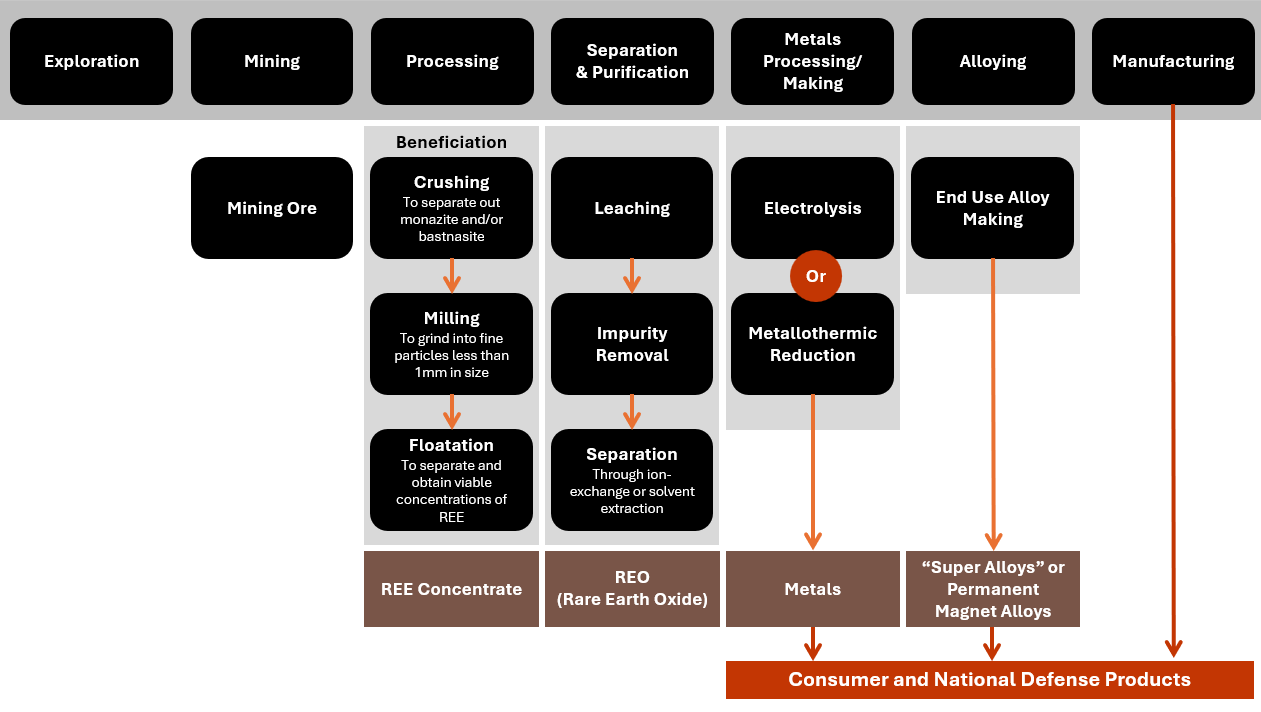
\includegraphics[width=1\linewidth]{Final_report_files/figure-latex/Critical_Mineral_Extraction_Process_v2} 

}

\caption{REE Value Chain (Source: US Department of Energy, 2017)}\label{fig:ree-vc}
\end{figure}

Recently, water-leaching is a prevailing approach since it mitigate the flaw from traditional techniques. Water leaching can be considered as less environmentally detrimental compared to strong acid/alkaline leaching, as well as cost effective for solvent selection. The crucial stages on this preparation workflow are low temperature activation and water leaching. During the stage of low temperature activation, the chemical reaction within coal fly ash (CFA) will be facilitated by complexation agents (ammonium salts or weak acids) in covered alumina crucibles, which help liberate critical elements from the matrix of the CFA. After the activation and cool down to ambient temperature, the tablets are placed in water for the leaching and dissolve process. Water acts as the leaching solvent, extracting these soluble elements into the leachate.The configuration in temperature and mass ratio of solvent will be the vital determinant for optimized recovery. Take Lithium example, it can achieve a stable leaching efficiency of 90\% through ammonium fluoride leaching at 150°C with a \(SiO_2/NH_4F\) mass ratio of 1:1.35 \textcite{Xu2021}.

Another innovation is Hydrophobic-Hydrophilic Separation (HHS), designed to leverages the disparity of affinity (water-repellent \& water-friendly) properties of substances to achieve separation.It can treat as a complementary application for small particle delamination without size limit, providing flexible and extensible purpose in the segregation of ultrafine coal \textcite{Hodgkinson2021}.

In precious \textcite{Hodgkinson2020} element mapping project on Bowen basin,the largest coal reserves in Australia, the concentration of element composition is subjective to sample's lithology rather than the depth grading:

1). In coal and derivative, albeit majority of element concentrations is inferior of the benchmark against earth crust average, local samples exhibit enrichment in HREE and Scandium in respect to \textcite{McLennan2011} Post-Archaean Australian Shales (PAAS) standard , while abnormal 4-6 times higher than crustal average in moderate critical element, Bismuth(Bi) .

2). Siltstone and mudstone has a lackluster finding to classify enrichment for majority of elements concentration,except for the concentration of Cobalt compound barely meet crustal average, whose ubiquitous economic value may warrant further examination.

3). As the sediment from volcanic ash, tuffaceous rock is rich in pumice and lithic fragments. The sample display a series of elevated concentrations of strategic elements including REE, Ga and Bi. Besides, a potential Lithium-rich borehole is found, with approximate 5 times higher than crustal average.

\hypertarget{objectives-and-significance}{%
\section{Objectives and Significance}\label{objectives-and-significance}}

\hypertarget{exploratory-data-analysis}{%
\section{Exploratory Data Analysis}\label{exploratory-data-analysis}}

\hypertarget{methodology}{%
\section{Methodology}\label{methodology}}

\hypertarget{results}{%
\section{Results}\label{results}}

\hypertarget{discussions}{%
\section{Discussions}\label{discussions}}

\hypertarget{conclusion}{%
\section{Conclusion}\label{conclusion}}

\hypertarget{appendix}{%
\section{Appendix}\label{appendix}}

\newpage

\printbibliography[title=Reference]

\end{document}
